\documentclass[12 pt]{exam}
\usepackage{graphicx, enumitem, amsmath, amssymb}
\graphicspath{ {./images/} }
\usepackage{tikz, pgfplots}
\pgfplotsset{compat=1.16}
\usetikzlibrary{shapes,arrows}
%\usepackage{Minion Pro}
\printanswers

\title{2.5 Short Run Profit Maximization - Practice Problems (Answers)}
\author{Ryan Safner}
\date{ECON 306 - Spring 2020}

\begin{document}

\maketitle

A firm has short-run costs given by:
$$\begin{aligned}
C(q)&=q^2+1\\
MC(q)&=2q\\ \end{aligned}$$

\begin{questions}

\question Write an equation for fixed costs, $f$.

\begin{solution}
Fixed costs are the part of the total cost function that do not change with output. Imagine if $q=0$ and the firm produced nothing, it would still have to pay \$1. 

\begin{equation*}
f=1	
\end{equation*}
\end{solution}

\question Write an equation for variable costs, $VC(q)$.

\begin{solution}

These are the terms of the cost function that change with output (have a variable in them). 

\begin{equation*}
VC(q)=q^2 	
\end{equation*}

\end{solution}

\question Write an equation for average fixed costs, $AFC(q)$.

\begin{solution}
\begin{equation*}
AFC(q)=\frac{C(q)}{q}=\frac{1}{q} 	
\end{equation*}

\end{solution}

\question Write an equation for average variable costs, $AVC(q)$.

\begin{solution}

\begin{equation*}
AVC(q)=\frac{VC(q)}{q}=\frac{q^2}{q} = q
\end{equation*}

\end{solution}
	
\question Write an equation for average (total) costs, $AC(q)$.

\begin{solution}

\begin{equation*}
AC(q)=\frac{C(q)}{q}=\frac{q^2+1}{q}=q+\frac{1}{q}
\end{equation*}

Alternatively:

$$\begin{aligned}
AC(q)&=AVC(q)+AFC(q)\\
AC(q)&=q+\frac{1}{q}\\	
\end{aligned}$$

\end{solution}

\question Suppose the firm is in a competitive market, and the current market price is \$4, how many units of output maximize profits?

\begin{solution}

The firm's profit maximizing quantity of output occurs where $MR(q)=MC(q)$. Since we know for a competitive firm, $MR(q)$ is the same is the price, we can set $p=MC(q)$ to solve for $q^*$: 

$$\begin{aligned}
	p=MR&=MC\\
	4&=2q\\
	q^*&=2 \\
\end{aligned}$$

\end{solution}

\clearpage 

\question How much profit will this firm earn?

\begin{solution}
Profit is total revenues minus total costs:

$$\begin{aligned}
	\pi &= R(q)-C(q)\\
	\pi &= pq-(q^2+1)	\\
	\pi &= (4)(2)-(2^2 + 1)	\\
	\pi &= (8)-(5)\\
	\pi &= \$3\\
\end{aligned}$$

Profits are \$3.
	
We could also calculate this using price and average cost: 

$$\begin{aligned}
	\pi &=q(p-AC(q))\\
	\pi &=q(p-\big[q+\frac{1}{q}\big])\\
	\pi &=2(4-\big[2+\frac{1}{2}\big])\\
	\pi &=2(4-[2.5])\\
	\pi &=2(1.5)\\
	\pi&=\$3\\ 
\end{aligned}$$
	
\begin{center} 
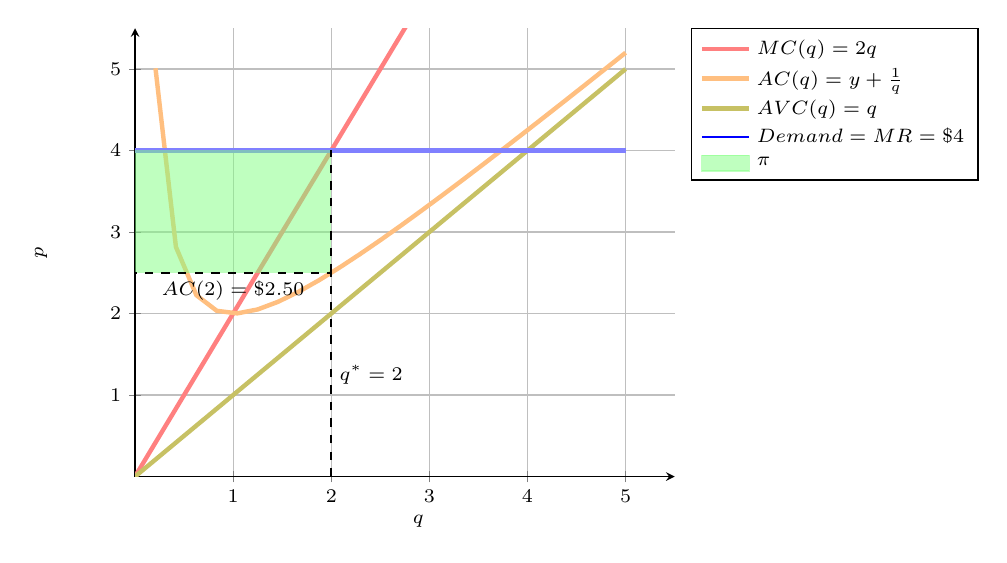
\begin{tikzpicture}\scriptsize 
	\begin{axis}[
		xlabel=$q$,
		ylabel=$p$,
		grid=major,
		legend pos=outer north east,
		legend cell align=left,
		axis lines=center,
		xtick={0,1,2,...,5},
		ytick={0,1,2,...,5},
		ymax=5,
		legend cell align=left,
		enlarge x limits={rel=0.1, upper},
		enlarge y limits={rel=0.1, upper},
		every axis y label/.style={at={(axis description cs:-0.2,0.5)},rotate=90,anchor=north},
		every axis x label/.style={at={(axis description cs:0.5,-0.1)},anchor=west},
		]
		\addplot[ultra thick, domain=0:5,red!50, samples=20]{2*x};
		\addlegendentry{$MC(q)=2q$}
		\addplot[ultra thick, domain=0:5,orange!50]{x+1/x};
		\addlegendentry{$AC(q)=y+\frac{1}{q}$}
		\addplot[ultra thick, domain=0:5,olive!50]{x};
		\addlegendentry{$AVC(q)=q$}
		\draw[blue!50, ultra thick] (axis cs:0,4)--(axis cs:5,4);
		\addlegendimage{blue, thick}
		\addlegendentry{$Demand=MR=\$4$}
		\addplot[green!50, opacity=0.5, fill=green!50, draw=none, area legend] coordinates{(0,2.5) (0,4) (2,4) (2,2.5)};
		\addlegendentry{$\pi$}
		\draw[thick, dashed] (axis cs:2,0)--node[right]{$q^*=2$}(axis cs: 2,2.5)--node[below]{$AC(2)=\$2.50$}(axis cs: 0,2.5);
		\draw[thick, dashed] (axis cs:2,2.5)--(axis cs: 2,4);
		%\addplot[thick, domain=0:5,black]{1/x};
		%\addlegendentry{$AFC(q)=\frac{10}{y}$}
		%\draw[blue, thick, dashed] (axis cs: 0,10)--(axis cs:8,10);
	\end{axis}
	\end{tikzpicture}
\end{center} 

We can see visually that profits (in green) are the area of the box between price \$4 and average cost at $q^*=2$, which is \$2.50. Thus, profit per unit is \$1.50, for two units, a total profit of \$3. 
	
\end{solution}

\clearpage

\question At what market price would the firm break even $(\pi=0)$?

\begin{solution}

A firm breaks even where profits are zero, and we know that is where price equals average cost. We want to find the lowest possible average cost, as that is the price that would produce no profits. Since price is marginal revenue, and the firm always sets $MR(q)=MC(q)$, we know that the minimum of the average cost curve is where it is equal to marginal cost, so we set: 

$$\begin{aligned}
	AC(q)&=MC(q)\\
	q+\frac{1}{q}&=2q	\\
	q^2+1&=2q^2	\\
	1&=q^2	\\
	1&=q^* \\
\end{aligned}$$

We know the quantity but we need to find the price where the firm breaks even, so plugging this back into either marginal cost or average cost: 

$$\begin{aligned}
	MC(q)&=2q\\
	MC(1)=2(1)\\
	MC(1)&=2\\
\end{aligned}$$

$$\begin{aligned}
	AC(q)&=q+\frac{1}{q}\\
	AC(1)=(1)+\frac{1}{(1)}\\
	AC(1)&=2\\
\end{aligned}$$

\begin{center} 
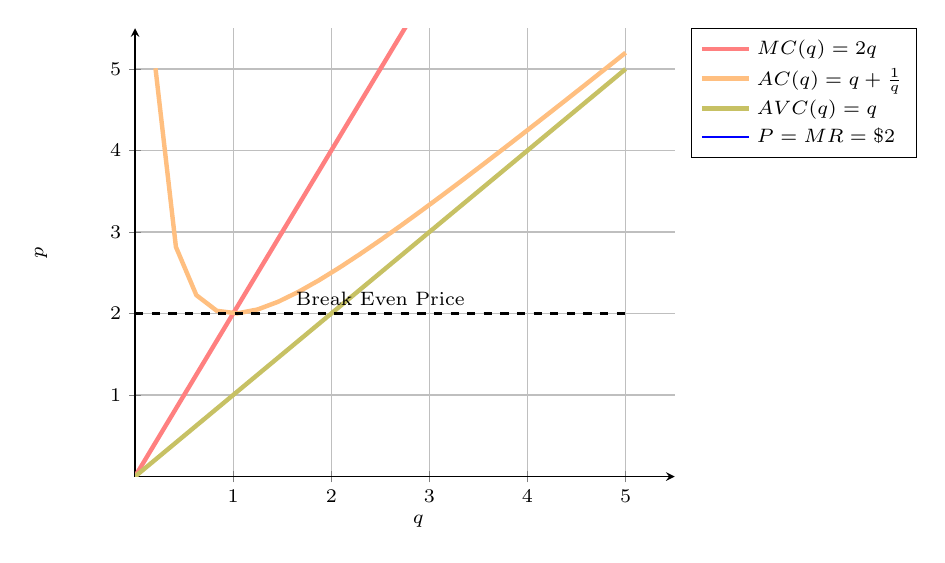
\begin{tikzpicture}\scriptsize 
	\begin{axis}[
		xlabel=$q$,
		ylabel=$p$,
		grid=major,
		legend pos=outer north east,
		legend cell align=left,
		axis lines=center,
		xtick={0,1,2,...,5},
		ytick={0,1,2,...,5},
		ymax=5,
		legend cell align=left,
		enlarge x limits={rel=0.1, upper},
		enlarge y limits={rel=0.1, upper},
		every axis y label/.style={at={(axis description cs:-0.2,0.5)},rotate=90,anchor=north},
		every axis x label/.style={at={(axis description cs:0.5,-0.1)},anchor=west},
		]
		\addplot[ultra thick, domain=0:5,red!50, samples=20]{2*x};
		\addlegendentry{$MC(q)=2q$}
		\addplot[ultra thick, domain=0:5,orange!50]{x+1/x};
		\addlegendentry{$AC(q)=q+\frac{1}{q}$}
		\addplot[ultra thick, domain=0:5,olive!50]{x};
		\addlegendentry{$AVC(q)=q$}
		\draw[thick, dashed] (axis cs:0,2)--node[above]{Break Even Price}(axis cs:5,2);
		\addlegendimage{blue, thick}
		\addlegendentry{$P=MR=\$2$}
		%\draw[thick, dashed] (axis cs:1,0)--node[right]{$q^*=1$}(axis cs: 1,2)--(axis cs: 0,2);
		%\addplot[thick, domain=0:5,black]{1/x};
		%\addlegendentry{$AFC(q)=\frac{10}{y}$}
		%\draw[blue, thick, dashed] (axis cs: 0,10)--(axis cs:8,10);
	\end{axis}
	\end{tikzpicture}
\end{center} 

\end{solution} 

\question Below what market price would the firm shut down in the short run if it were earning losses? 

\begin{solution}
A firm shuts down in the short run when it can no longer cover its average variable costs. We know the minimum average variable cost happens when it is equal to marginal cost:

$$\begin{aligned}
	AVC(q) &= MC(q)\\
	q &= 2q\\
	q&=0	\\
\end{aligned}$$

Where $q=0$, price is $MC(0)=2(0)=\$0$.

\end{solution}

\question Write out the firm's short run supply function.

\begin{solution}

$$\begin{aligned}
	p=MR&=MC\\	
	p&=2q\\
	q&=\frac{1}{2}p\\
\end{aligned}$$

\begin{center} 
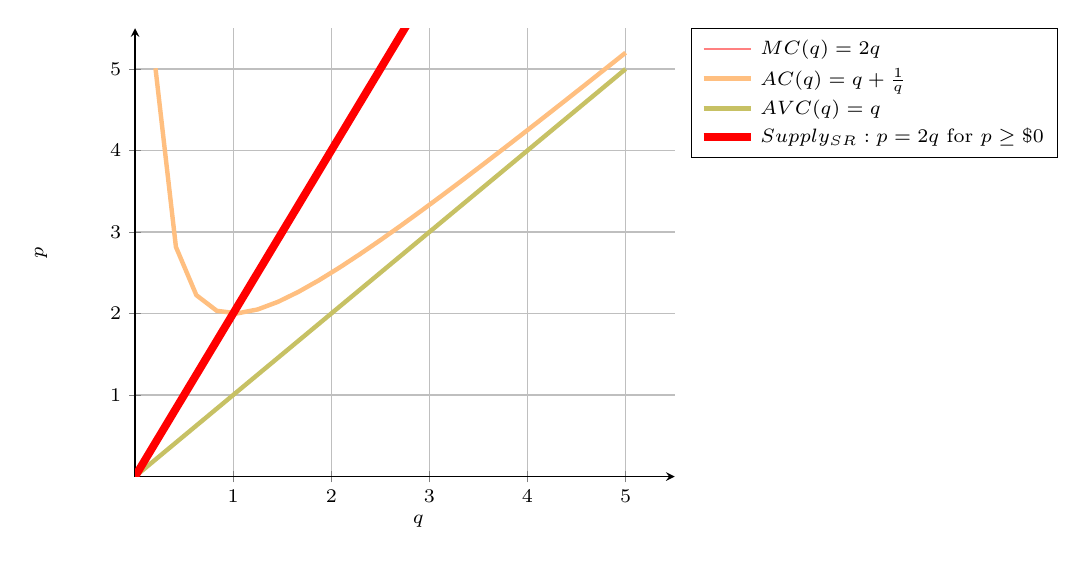
\begin{tikzpicture}\scriptsize 
	\begin{axis}[
		xlabel=$q$,
		ylabel=$p$,
		grid=major,
		legend pos=outer north east,
		legend cell align=left,
		axis lines=center,
		xtick={0,1,2,...,5},
		ytick={0,1,2,...,5},
		ymax=5,
		enlarge x limits={rel=0.1, upper},
		enlarge y limits={rel=0.1, upper},
		every axis y label/.style={at={(axis description cs:-0.2,0.5)},rotate=90,anchor=north},
		every axis x label/.style={at={(axis description cs:0.5,-0.1)},anchor=west},
		]
		\addplot[thick, domain=0:5,red!50, samples=20]{2*x};
		\addlegendentry{$MC(q)=2q$}
		\addplot[ultra thick, domain=0:5,orange!50]{x+1/x};
		\addlegendentry{$AC(q)=q+\frac{1}{q}$}
		\addplot[ultra thick, domain=0:5,olive!50]{x};
		\addlegendentry{$AVC(q)=q$}
		\addplot[line width=0.1cm, domain=0:5,red, samples=20]{2*x};
		\addlegendentry{$Supply_{SR}: p=2q$ for $p \geq \$0$}		
		%\addplot[thick, domain=0:5,black]{1/x};
		%\addlegendentry{$AFC(q)=\frac{10}{y}$}
		%\draw[blue, thick, dashed] (axis cs: 0,10)--(axis cs:8,10);
	\end{axis}
	\end{tikzpicture}
\end{center} 

$$\begin{aligned}
				\text{Firm's Short Run Inverse Supply}&= \left\{
 		 \begin{array}{ll}
    		p=MC(q) & \text{if } p \geq AVC(q) \\
   			q=0 & \text{if } p < AVC(q)\\
  		\end{array}
  		\right. 	\\
  						&= \left\{
 		 \begin{array}{ll}
    		p=2q & \text{if } p \geq \$0 \\
   			q=0 & \text{if } p < \$0\\
  		\end{array}
  		\right. 	\\
\end{aligned}$$

If you wanted to write the firm's supply curve (instead of the inverse), solve for $q$ to get: 

\begin{equation*}
	q=\frac{1}{2}p \text{ for }p \geq 0
\end{equation*}

In the long run, the firm only produces when it is profitable to do so, i.e. $p \geq AC(q)$. So the supply curve is the region of the $MC(q)$ curve above the minimum $AC(q)$. 	

$$\begin{aligned}
				\text{Firm's Long Run Inverse Supply}&= \left\{
 		 \begin{array}{ll}
    		p=MC(q) & \text{if } p \geq AC(q) \\
   			q=0 & \text{if } p < AC(q)\\
  		\end{array}
  		\right. 	\\
  						&= \left\{
 		 \begin{array}{ll}
    		p=2q & \text{if } p \geq \$2 \\
   			q=0 & \text{if } p < \$2\\
  		\end{array}
  		\right. 	\\
\end{aligned}$$

\begin{center} 
		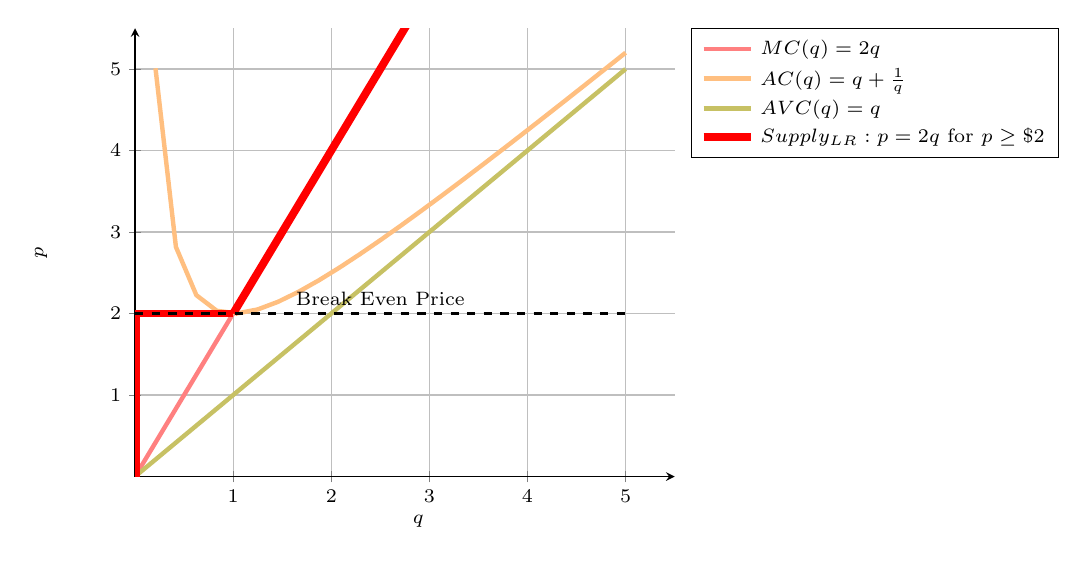
\begin{tikzpicture}\scriptsize 
	\begin{axis}[
		xlabel=$q$,
		ylabel=$p$,
		grid=major,
		legend pos=outer north east,
		legend cell align=left,
		axis lines=center,
		xtick={0,1,2,...,5},
		ytick={0,1,2,...,5},
		ymax=5,
		legend cell align=left,
		enlarge x limits={rel=0.1, upper},
		enlarge y limits={rel=0.1, upper},
		every axis y label/.style={at={(axis description cs:-0.2,0.5)},rotate=90,anchor=north},
		every axis x label/.style={at={(axis description cs:0.5,-0.1)},anchor=west},
		]
		\addplot[ultra thick, domain=0:5,red!50, samples=20]{2*x};
		\addlegendentry{$MC(q)=2q$}
		\addplot[ultra thick, domain=0:5,orange!50]{x+1/x};
		\addlegendentry{$AC(q)=q+\frac{1}{q}$}
		\addplot[ultra thick, domain=0:5,olive!50]{x};
		\addlegendentry{$AVC(q)=q$}
		\addplot[line width=0.1cm, domain=1:5,red, samples=20]{2*x};
		\addlegendentry{$Supply_{LR}: p=2q$ for $p \geq \$2$}		
		\draw[line width=0.1cm, red] (axis cs:0.01,0)--(axis cs:0.01,2)--(axis cs:1,2);
				\draw[thick, dashed] (axis cs:0,2)--node[above]{Break Even Price}(axis cs:5,2);

		%\addplot[thick, domain=0:5,black]{1/x};
		%\addlegendentry{$AFC(q)=\frac{10}{y}$}
		%\draw[blue, thick, dashed] (axis cs: 0,10)--(axis cs:8,10);
	\end{axis}
	\end{tikzpicture}
	\end{center} 

The long run equilibrium price must be equal to average cost, so there are no profits or losses to induce entry or exit. We've seen this happens at \$2.

\end{solution}

\end{questions}

\end{document}